\section{Hardware description}
\label{sec:hw-description}

Steistat is a single-channel, three-electrode potentiostat built directly
from the Analog Devices AD5940/AD5941 datasheet~\cite{devices2024ad5940},
standard three-electrode potentiostat design practice, and the Analog
Devices AD5940 evaluation-kit reference firmware~\cite{ad5940_examples_github}.

\subsection{Instrument}
\label{sec:device-photo}
Figure~\ref{fig:device-photo} shows the assembled instrument used for
every measurement in this paper: the AD5941 AFE and Seeed Studio XIAO
RP2040 MCU on the \texttt{STEI\_Bstat\_v1.2} carrier board (\SI{45.0}{}
$\times$ \SI{60.0}{\milli\metre}), with the working/reference/counter
(WE/RE/CE) electrode header used to connect the dummy cell.

\begin{figure}[H]
\centering
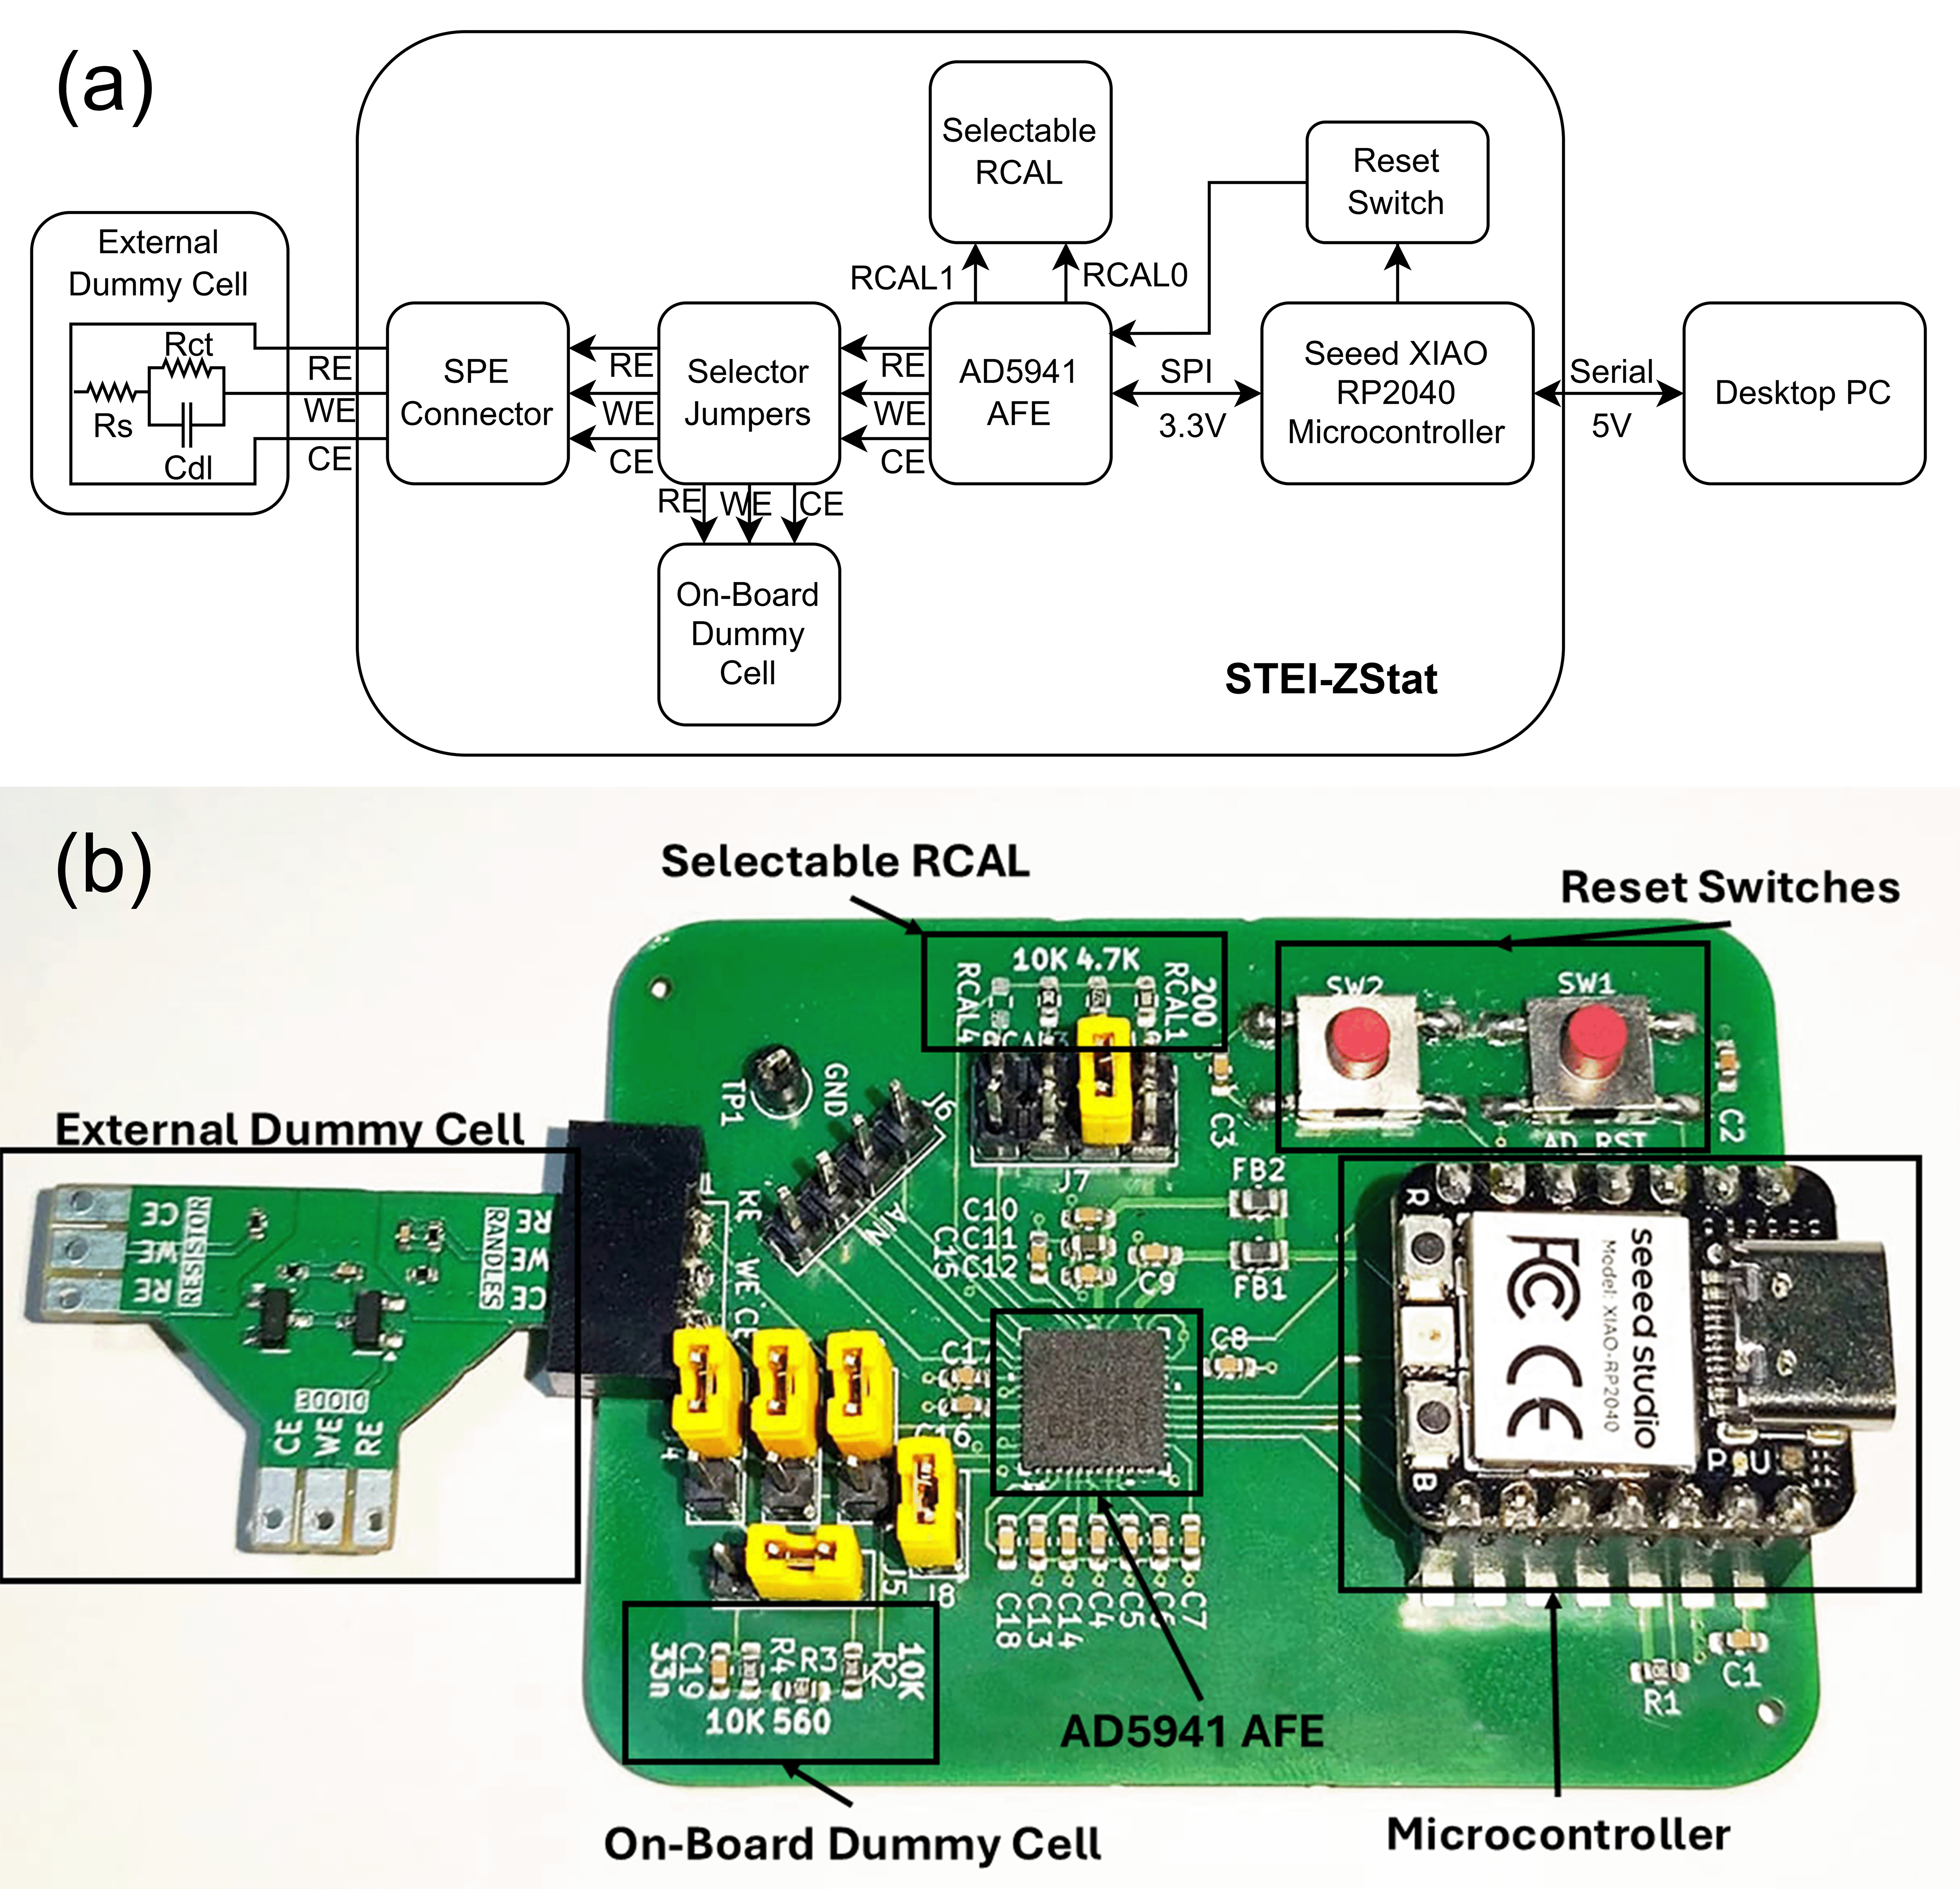
\includegraphics[width=0.85\linewidth]{./figures/fig1_STEI-ZStat.png}
\caption{Steistat, the AD5941/RP2040 potentiostat under test: assembled
board with the AD5941 AFE, XIAO RP2040 MCU, and WE/RE/CE electrode header
used to connect the dummy cell of Section~\ref{sec:protocol}.}
\label{fig:device-photo}
\end{figure}

\subsection{Components}
\label{sec:components}
Table~\ref{tab:components} lists the instrument's principal components
(the full itemized Bill of Materials is given in
Section~\ref{sec:bom}). The AD5941 supplies the entire analog measurement
chain -- both excitation loops, both transimpedance stages, the ADC, and
the DFT engine -- as characterized, off-the-shelf silicon~\cite{devices2024ad5940};
the RP2040 MCU is responsible only for register sequencing, host
communication, and unit conversion. This is exactly why the eleven defects
diagnosed in this paper (Section~\ref{sec:validation}) are firmware
defects, not analog ones: each is a matter of which of the AD5941's own,
correctly-functioning internal paths and states the firmware asks for, how
it declares the on-board calibration resistor it measures against, and how
it interprets the codes and results those paths return.

\begin{table}[h]
\centering
\footnotesize
\setlength{\tabcolsep}{4pt}
\caption{Principal components of the Steistat instrument.}
\label{tab:components}
\begin{threeparttable}
\begin{tabular}{@{}p{0.24\linewidth}p{0.68\linewidth}@{}}
\toprule
Component & Role / key specification \\
\midrule
Electrochemical AFE & Analog Devices AD5941: LP loop (12-bit LPDAC + 6-bit
  $V_{\mathrm{zero}}$ DAC, LPPA, LPTIA with a switchable feedback resistor,
  $\Rtia$: \SI{110}{\ohm}--\SI{160}{\kilo\ohm} for DC/staircase methods) and
  HS loop (12-bit HSDAC, HSTIA) for AC/impedance excitation; 16-bit
  $\Sigma\Delta$ ADC and hardware DFT accelerator shared by
  both~\cite{devices2024ad5940} \\
Microcontroller & Seeed Studio XIAO RP2040 (dual-core Cortex-M0+); runs
  the register-sequencing firmware and the USB-CDC host interface \\
MCU--AFE link & Bit-banged SPI (custom XIAO pin map; native SPI0 pinout
  not used), effective clock in the hundreds of kHz, well under the
  AD5941's rated \SI{12}{\mega\hertz}~\cite{devices2024ad5940} \\
Calibration resistor ($\Rcal$) & \SI{200}{\ohm} (\texttt{RCAL1}) fitted on
  the \texttt{STEI\_Bstat\_v1.2} carrier board; the reference the AFE
  measures against to calibrate its own transimpedance gain -- the firmware
  had declared this as \SI{10}{\kilo\ohm} (Defect~D-RCAL, Section~\ref{sec:otherdefects}) \\
LPTIA topology select (\texttt{k}) & Runtime-selectable feedback-resistor
  code and filter-bypass switch (bit0: SW13; bits1--3: LPTIARF code),
  added during this work to characterize the DC signal chain on hardware
  without reflashing \\
Host interface & USB-CDC virtual serial, ASCII single-letter command
  protocol, \SI{1}{\mega baud} (full grammar in Section~\ref{sec:operation}) \\
Electrode/load interface & 3-terminal working/reference/counter (WE/RE/CE)
  connector; accepts either an electrochemical cell or the passive dummy
  cell of Section~\ref{sec:protocol} \\
\bottomrule
\end{tabular}
\end{threeparttable}
\end{table}

\subsection{Signal routing: two loops, one AFE}
\label{sec:loop-diagram}
Figure~\ref{fig:loop-diagram} shows the routing that
Section~\ref{sec:rootcause}'s Defect 1 got wrong. Every Analog
Devices reference example for a DC/staircase method -- including
\texttt{AD5940\_ChronoAmperometric}, \texttt{AD5940\_SqrWaveVoltammetry},
and \texttt{AD5940\_Ramp} (which this project's own, already-working
legacy CV engine is derived from) -- routes through the LP loop; only the
EIS implementation, which needs the HSDAC's sinusoidal waveform generator,
uses the HS loop~\cite{ad5940_examples_github}. Prior to the fix reported
in this paper, \texttt{C\_CA}, \texttt{C\_SWV}, and \texttt{C\_DPV}
instead configured the HS loop -- the lower branch of
Figure~\ref{fig:loop-diagram} -- which is a real, correctly-functioning
AD5941 capability, just the wrong one for a DC potential-step measurement.

\begin{figure}[H]
\centering
\resizebox{\linewidth}{!}{%
\begin{tikzpicture}[
  block/.style={draw, rounded corners, minimum height=1.1cm,
    minimum width=3.1cm, align=center, font=\small},
  arr/.style={-{Latex[length=2mm]}, thick},
  edgelabel/.style={font=\scriptsize, align=center, text width=2.1cm}
]
\node[block] (cmd1) {CA, CV, SWV, DPV,\\OCP command};
\node[block, right=3.1cm of cmd1] (lp) {LP loop\\(LPDAC + LPPA + LPTIA)};
\node[block, below=1.6cm of cmd1] (cmd2) {EIS command};
\node[block, right=3.1cm of cmd2] (hs) {HS loop\\(HSDAC + HSTIA)};
\node[block, right=2.9cm of lp, yshift=-0.8cm] (cell) {Electrode /\\dummy cell};

\draw[arr] (cmd1) to node[midway, above, edgelabel] {LP loop\\(this paper's fix)} (lp);
\draw[arr] (cmd2) to node[midway, below, edgelabel] {HS loop\\(unchanged)} (hs);
\draw[arr] (lp) to[bend left=8] (cell);
\draw[arr] (hs) to[bend right=8] (cell);
\end{tikzpicture}%
}
\caption{Steistat's two AD5941 excitation/sensing loops and which
electrochemical methods use each. Before the fix in
Section~\ref{sec:rootcause}, CA, SWV, and DPV incorrectly routed through
the HS loop (the path correctly used only by EIS); the fix moves them onto
the LP loop, matching every Analog Devices DC-method reference
example~\cite{ad5940_examples_github}. OCP and CV use the LP loop through
their own, independently-correct code paths that this defect never
touched.}
\label{fig:loop-diagram}
\end{figure}

\subsection{Software architecture}
\label{sec:swarch}
The firmware sketch (\texttt{AD5941\_25.ino}) instantiates three top-level
objects at boot: \texttt{C\_DataStorage} (a centralized parameter store),
\texttt{C\_Communication} (the serial command parser/dispatcher), and
\texttt{C\_AD5941\_Setup} (chip initialization). \texttt{C\_Communication}
owns the ASCII command grammar (Section~\ref{sec:operation}) and, on
receiving a method-run command, instantiates and drives the corresponding
method class (\texttt{C\_CA}, \texttt{C\_SWV}, \texttt{C\_DPV},
\texttt{C\_EIS}, \texttt{C\_OCP}, \texttt{C\_CV}), each bound to the shared
\texttt{C\_DataStorage} instance via a raw pointer.

\subsection{Object-oriented design}
\label{sec:oop}
A source-level audit originally found the firmware's eight C++ classes
(\texttt{C\_CA}, \texttt{C\_DPV}, \texttt{C\_SWV}, \texttt{C\_EIS},
\texttt{C\_OCP}, \texttt{C\_Communication}, \texttt{C\_DataStorage}, and
\texttt{C\_AD5941\_Setup}) exhibited real but limited object orientation:
\texttt{C\_DataStorage} was entirely public fields wearing a
\texttt{class} keyword, not an encapsulating abstraction; only
\texttt{C\_Communication} and \texttt{C\_AD5941\_Setup} had genuine
encapsulated state; no inheritance, virtual functions, or interface
abstraction appeared anywhere in the project's own code; cyclic voltammetry
was not a class at all; and \texttt{C\_CA::ConfigDCMeasurement()},
\texttt{C\_SWV::ConfigDCMeasurement()}, and \texttt{C\_DPV::ConfigDCMeasurement()}
were verbatim-duplicated, together with a fourth, unreachable copy in a
dead free-function file, \texttt{electrochemical\_methods.cpp}. That
duplication was not merely a maintainability concern in the abstract:
several of the eleven defects Section~\ref{sec:validation} diagnoses, having
been made once, existed as three or four literal repetitions and had to be
found and fixed that many times over.

This paper closes every one of those gaps directly, not only the
duplication. Two structural changes were made, verified not to change any
reported measurement (Section~\ref{sec:validation} reproduces this paper's
own CV accuracy figure, unchanged, after both):
\begin{itemize}
\item \textbf{A shared polymorphic interface for all six methods.} A new
  abstract base, \texttt{C\_ElectrochemicalMethod}, declares a pure-virtual
  \texttt{Run()} and a virtual \texttt{Begin(C\_DataStorage*)}. The
  previously-introduced \texttt{C\_DCPotentiostatMethod} (which
  \texttt{C\_CA}, \texttt{C\_SWV}, and \texttt{C\_DPV} inherit, and which
  now carries their formerly-duplicated configuration, sampling, and
  conversion logic register-for-register and formula-for-formula) now
  itself inherits from this base, as do \texttt{C\_EIS} and \texttt{C\_OCP}
  directly. \texttt{C\_OCP} gained a \texttt{Run()} that composes its
  existing \texttt{Configure()}/\texttt{Measure()} calls, matching the
  shape every other method class already had; its separate
  \texttt{Calculate()}-only calibration path is untouched. Cyclic
  voltammetry, previously outside the class structure entirely, is now
  wrapped in a new \texttt{C\_CV} class whose \texttt{Run()} performs
  exactly the parameter synchronization and legacy-engine call
  (\texttt{cvSetup()}) that the dispatcher used to do inline -- no change
  to \texttt{cv.cpp}/\texttt{rampTest.cpp}'s own sweep logic (which is
  also why, as Figure~\ref{fig:loop-diagram} notes, that sweep logic was
  never exposed to the loop-routing and ADC-convention defects
  Section~\ref{sec:validation} diagnoses -- it does, however, carry two
  of its own defects, Section~\ref{sec:rootcause}, found by the same
  diagnostic process). Every \texttt{C\_Communication::Dispatch<Method>()}
  call site now follows the same shape: construct, \texttt{Begin(m\_pData)},
  \texttt{Run()}. The dead free-function duplicate in
  \texttt{electrochemical\_methods.cpp} was removed.
\item \textbf{Field-level encapsulation of \texttt{C\_DataStorage}.} All
  fields are now private, each with a paired \texttt{Get<Field>()}/
  \texttt{Set<Field>()} accessor; the roughly 150 direct-field-access call
  sites across \texttt{communication.cpp} and the five method-class
  \texttt{.cpp} files were updated to match, one file at a time, with a
  clean compile after every file as the correctness check -- a missed site
  is a compile error, not a silent bug, under this specific migration.
\end{itemize}
Nine classes now exist. All six electrochemical-method classes sit under
one polymorphic hierarchy with a genuine base/derived relationship and a
pure-virtual interface; \texttt{C\_DataStorage} is encapsulated by the
standard definition (private state, accessed only through its own
methods); and cyclic voltammetry participates in the class structure like
every other method. This paper does not claim the result is a
maximally-abstracted architecture -- there is still exactly one
inheritance level, no polymorphic dispatch through base-class pointers at
the call sites themselves (each \texttt{Dispatch<Method>()} still names its
concrete class directly), and \texttt{C\_DataStorage}'s accessors are
mechanical get/set pairs rather than a richer domain interface -- but every
finding the original audit raised against these two classes'
categories (encapsulation, inheritance/polymorphism, duplication) has been
addressed, verified against this paper's own hardware-measured CV accuracy
result rather than left as a documented gap.

\subsection{Electrochemical measurement methods}
\label{sec:methodstable}
Six methods are implemented: OCP, CV, CA, SWV, DPV, and EIS.
Table~\ref{tab:methods} summarizes their implementation and validated
status on this firmware (Section~\ref{sec:validation}).

\begin{table}[H]
\centering
\footnotesize
\setlength{\tabcolsep}{4pt}
\caption{Electrochemical methods, implementation, and validated status.}
\label{tab:methods}
\begin{tabular}{@{}p{0.9cm}p{2.6cm}p{3.6cm}@{}}
\toprule
Method & Implementation & Status \\
\midrule
OCP & \texttt{C\_OCP} (LP loop, direct read) & Not independently
  validated on this baseline (Section~\ref{sec:discussion}) \\
CV & \texttt{C\_CV}, wrapping \texttt{cv.cpp}/\allowbreak\texttt{rampTest.cpp} (LP loop, \texttt{AD5940\_Ramp}-derived) & Validated: $R^2\geq0.999998$,
  $+0.427\,\%$ recovered-resistance error (Section~\ref{sec:validation}) \\[7pt]
CA & \texttt{C\_CA} (LP loop, fixed this work) & Step-onset current
  correctly signed and monotonic; sustained current does not track
  potential (Section~\ref{sec:discussion}) \\
SWV & \texttt{C\_SWV} (LP loop, fixed this work) & Smooth, bounded
  differential current; same sustained-current caveat as CA \\
DPV & \texttt{C\_DPV} (LP loop, fixed this work) & Smooth, bounded
  differential current; same sustained-current caveat as CA \\
EIS & \texttt{C\_EIS} (HS loop) & Not re-tested in this paper
  (Section~\ref{sec:discussion}) \\
\bottomrule
\end{tabular}
\end{table}

\subsection{Operating parameters}
\label{sec:params}
Table~\ref{tab:params} collects the parameters a user needs to operate
this instrument within its characterized range, derived directly from
Eqs.~\eqref{eq:vzero}--\eqref{eq:current}, the $\Rtia$ codes of
Table~\ref{tab:rtia}, and the AD5940 datasheet~\cite{devices2024ad5940}.
Current range and resolution are given for the two extreme $\Rtia$ codes
and for this project's default ($\Rtia=\SI{10}{\kilo\ohm}$), all at the
unity ADC gain (\texttt{ADCPGA\_1}) this firmware uses; a full-scale
current in Eq.~\eqref{eq:current} corresponds to
$I=V_{\mathrm{ref}}/(\mathrm{PGA}\cdot\Rtia)$ and one ADC code (LSB) to
that value divided by $32768$.

\begin{table}[H]
\centering
\footnotesize
\setlength{\tabcolsep}{4pt}
\caption{Operating parameters.}
\label{tab:params}
\begin{tabular}{@{}p{3.3cm}p{4.3cm}@{}}
\toprule
Parameter & Value \\
\midrule
Applied-potential resolution & \SI{0.537}{\milli\volt} per DAC code
  (Eq.~\eqref{eq:vbias}) \\
Working-electrode bias ($V_{\mathrm{zero}}$) & Fixed at \SI{1100}{\milli\volt},
  not user-configurable in this firmware (Section~\ref{sec:rootcause}) \\
Rated excitation amplitude & Up to \SI{1.2}{\volt}$_{pp}$~\cite{devices2024ad5940} \\
Current range ($\Rtia=\SI{110}{\ohm}$ to $\SI{160}{\kilo\ohm}$,
  Table~\ref{tab:rtia}) & Full-scale $\approx\SI{16.5}{\milli\ampere}$ down
  to $\approx\SI{11.4}{\micro\ampere}$ \\
Current resolution, default setting ($\Rtia=\SI{10}{\kilo\ohm}$) &
  $\approx\SI{5.6}{\nano\ampere}$ per ADC code \\
ADC & 16-bit $\Sigma\Delta$, offset-binary around raw code $0{\times}8000$
  (Section~\ref{sec:adcfix}) \\
Sample-rate ceiling & $\approx\SI{75}{\hertz}$ per conversion
  ($\geq\SI{13.3}{\milli\second}$ settling, Section~\ref{sec:validation});
  this firmware's own \SI{100}{\hertz} default sample-rate setting exceeds
  that ceiling \\
EIS frequency range (AFE-rated) & \SIrange{0.015}{200000}{\hertz}~\cite{devices2024ad5940} \\
Host interface & USB-CDC, ASCII commands, \SI{1}{\mega baud}
  (Section~\ref{sec:components}) \\
CV accuracy (this paper, Randles cell) & $R^2\geq0.999998$;
  $+0.427\,\%$ recovered-resistance error, $n=5$ replicate sweeps
  (Section~\ref{sec:validation}) \\
CV repeatability (this paper) & $\%\mathrm{RSD}=0.0084\,\%$ (Section~\ref{sec:validation}) \\
\bottomrule
\end{tabular}
\end{table}
